\documentclass[margin=5pt]{standalone}
\usepackage{array}
\usepackage{amsmath,amssymb}
\usepackage{tikz}
\usetikzlibrary{arrows}
\usetikzlibrary{shapes}
\usetikzlibrary{backgrounds}
\usetikzlibrary{patterns}
\usetikzlibrary{positioning}
\begin{document}
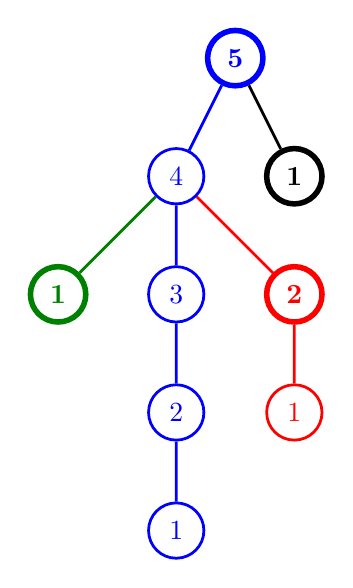
\begin{tikzpicture}[every node/.style={minimum width=2em,draw,circle,line width=1pt},
        edge from parent/.style=
        {draw,line width=1pt,edge from parent path={(\tikzparentnode) -- (\tikzchildnode)}},
        level distance=1.5cm,
        sibling distance=1.5cm,
        start/.style={line width=2pt,font=\bf},
        green/.style={color=green!50!black},
        red/.style={color=red},
        blue/.style={color=blue},
  ]

    \node[start,blue] {5}
    child[blue] {
        node[blue] {4}
        child[green] {
            node[start] {1}
        }
        child[blue] {
            node[] {3}
            child[] {
                node[] {2}
                child[] {
                    node[] {1}
                }
            }
        }
        child[red] {
            node[start] {2}
            child[] {
                node[] {1}
            }
        }
    }
    child {
        node[start] {1}
    };
\end{tikzpicture}
\end{document}
